\subsection{Worked Example}
\label{sec:station-example}

Table~\ref{tab:station-chain} gives the chain of the example station (Section~\ref{sec:example-data}) at
$P_{pcc} = -1000$\,MW: voltage, active and reactive power and current at the output of each element and the losses
of that element. The station delivers $P_{dc} = \exPdc$\,MW at its DC terminal with $I_d = \exId$\,kA; the losses
are $\exLoss$\,MW and the efficiency is $\exEta$\,\%. The modulation index is $m = \exM$ and the converter DC voltage
$U_{dpe\_conv} = \exUconv$\,kV. Table~\ref{tab:station-losses} splits the losses by element, and
Figure~\ref{fig:station-sld} shows the same results in the single-line diagram of the station.

\begin{table}[!ht]
  \centering
  \small
  \begin{tabularx}{\linewidth}{@{}>{\raggedright\arraybackslash}X r r r r r@{}}
    \toprule
    \textbf{Element (output)} & \multicolumn{1}{c}{\textbf{$U$ [kV]}} & \multicolumn{1}{c}{\textbf{$P$ [MW]}}
      & \multicolumn{1}{c}{\textbf{$Q$ [Mvar]}} & \multicolumn{1}{c}{\textbf{$I$ [kA]}}
      & \multicolumn{1}{c}{\textbf{$P_{loss}$ [MW]}} \\
    \midrule
    \tablerows{station/fig/chain_table}
    \bottomrule
  \end{tabularx}
  \caption{Station chain of the example at $P_{pcc} = -1000$\,MW, $U_{dpe} = 400$\,kV, $P_{aux} = 500$\,kW. AC rows:
           voltage line-to-line, current per converter on the valve side; arm reactor row: internal converter
           voltage and arm current (RMS); DC rows: voltage pole-to-ground, DC current, converter row with the sign of
           the convention}
  \label{tab:station-chain}
\end{table}

\begin{table}[!ht]
  \centering
  \small
  \begin{tabular}{@{}l r r@{}}
    \toprule
    \textbf{Part} & \multicolumn{1}{c}{\textbf{MW}} & \multicolumn{1}{c}{\textbf{\% of $|P_{pcc}|$}} \\
    \midrule
    \tablerows{station/fig/losses_table}
    \bottomrule
  \end{tabular}
  \caption{Loss breakdown of the example station}
  \label{tab:station-losses}
\end{table}

\begin{figure}[!ht]
  \centering
  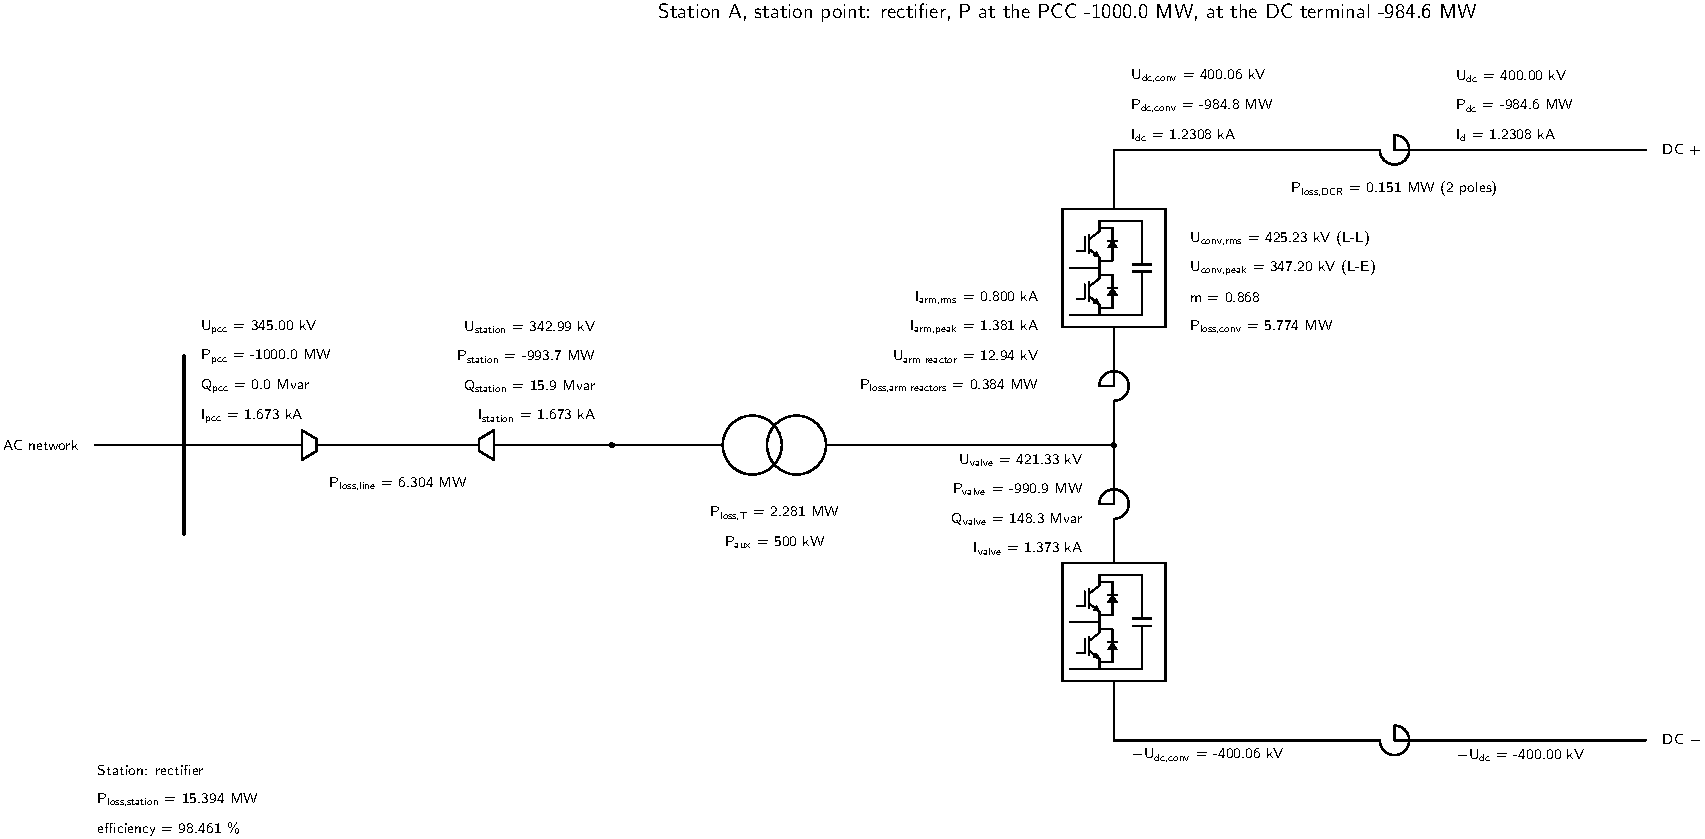
\includegraphics[width=\linewidth]{station/fig/loadflow_station.pdf}
  \caption{Single-line diagram of the example station with the results of Table~\ref{tab:station-chain}}
  \label{fig:station-sld}
\end{figure}

Table~\ref{tab:station-procedures} compares the two solution procedures of Section~\ref{sec:station-procedures}.
The DC power of the first row, given at the DC terminal, reproduces the PCC power after 4 secant iterations. The
third row is an inverter with $P_{dc} = 990$\,MW.

\begin{table}[!ht]
  \centering
  \small
  \begin{tabular}{@{}l r r r r r@{}}
    \toprule
    \textbf{Power given} & \multicolumn{1}{c}{\textbf{$P_{pcc}$ [MW]}} & \multicolumn{1}{c}{\textbf{$P_{dc}$ [MW]}}
      & \multicolumn{1}{c}{\textbf{$I_d$ [kA]}} & \multicolumn{1}{c}{\textbf{$U_{dpe\_conv}$ [kV]}}
      & \multicolumn{1}{c}{\textbf{Iterations}} \\
    \midrule
    \tablerows{station/fig/procedures_table}
    \bottomrule
  \end{tabular}
  \caption{Active power given at the PCC and at the station DC terminal; iterations of the secant method}
  \label{tab:station-procedures}
\end{table}
\FloatBarrier
